\section{Planning}
\subsection{Planning Methodology}
\glsreset{mdp}
\newacronym{pomdp}{POMDP}{Partially Observable Markov Decision Process}
\newacronym{nomdp}{NOMDP}{Non-Observable Markov Decision Process}
Our data transfer decision framework is designed to use intelligent planning
techniques to make real time decisions on data transfers within an organizations cloud
network. Examples of these techniques are \gls{mdp}, \gls{pomdp}, and \gls{nomdp}.
The purpose of these techniques is to provide a mathematical framework
to model decision making. Consider the scenario of a user (node) in an
organization wanting to send classified data to another user (node) in the cloud
environment. The sender has no idea if the recipient is trustworthy enough to
handle such critical files. The current common practice of using static policies to
guide decision making is not sufficient as it is infeasible to enumerate all
possible policies for all possible scenarios. Moreover generating run time
decisions through policies is slow. Thus, there exists a need for a dynamic,
real-time decision making process to address these problems. 
\FloatBarrier
\begin{figure}[h!]
    \label{fig:SystemBlockDiagram}
    \begin{center}
        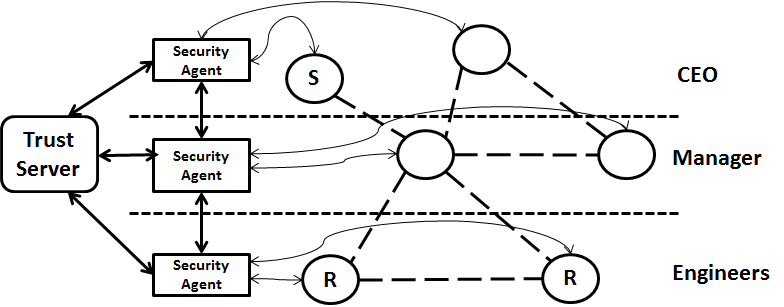
\includegraphics[width=0.95\textwidth]{Figures/Planning_Figure_1.png}
        \caption{System Block Diagram}
    \end{center}
\end{figure}
\FloatBarrier
We address these issues using intelligent planning techniques. The planning
algorithms in our framework make decisions based on probabilistic values which
are estimated from the trust values of users/nodes in a stochastic environment
\autocite{JMarecki2012}, \autocite{JWu.2011}. The algorithms then consider the classification level
of the document and the trust metric of the specific user(s) who are to receive
the classified documents. Using this the algorithm generates plans which will specify whether the
user/node is really trustworthy enough to handle such data.  

In the process of
developing the algorithm, we have explored three kinds of models: \gls{mdp},
\gls{pomdp}, and \gls{nomdp}. Initially the plan was to use a \gls{pomdp} as the 
primary decision maker in the
framework, since it is able to factor uncertainty into the decision making process.
Uncertainty arises from the fact that all the states (the model) of the cloud
environment is not always known or observable. However, after careful research
in this area we decided not to pursue using a \gls{pomdp} because the
\gls{pomdp} complexity
is very high \autocite{LeslieP.Kaelbling1998}, \autocite{Zilberman},
\autocite{DongNguyen2009}. 
That is, computationally, it is very expensive and the
process requires a lot of time to generate decisions, which would eventually
result in poor performance, which is generally unacceptable in today's fast paced, heavily interconnected organizational networks.
Alternatively, the solution is to use \gls{mdp} to make the decisions. In order
to use an \gls{mdp} however, all uncertainty needs to be removed from the system.
Hence, we make the assumption that all the states and the entirety of
the cloud environment is known and observable. Realistically, this is a valid
assumption, because in an organization all nodes should be known and the structure of nodes
is generally well defined. As a real world example, this translates to the organization's IT
manager knowing all the workstations and network connections within the
company. This is a well controlled inventory.

Now let us explore the structure of the \gls{mdp}. It
is a four tuple in total $< S, A, T, R >$ \autocite{QimingHe2000}:
\begin{description}
    \item{\textbf{S (States):}} Represents a finite set of states present in the cloud Environment.
    \item{\textbf{A (Actions):}} Represents a finite set of actions that are possible in
        every state $S_n$ of the cloud environment.
    \item{\textbf{T (Transition Function):}} Represents the probabilistic values of the occurrence of every action from every state. This can be derived from the known model/structure of the cloud environment.
    \item{\textbf{R (Reward/ Cost function):}} Represents Reward value at each state, which
    in our case is the trust value of every node/user.  
\end{description}
The \gls{mdp} tuple above is 
specifically modeled and/or changed to meet the requirements for the CloudAssure
framework. In addition to the above tuple, in order for the \gls{mdp} to operate we require a start
state and a goal state. Once a user/node makes a request to transfer data
to another user/node, a Security Agent takes over to process the request. Security Agents are comprised of special software that runs on an existing or dedicated server to perform and aid in various processes performed by the CloudAssure framework.

In the CloudAssure framework, the Security Agent's police the traffic and communicate with other Security Agents. 
The next step in the decision making process is for the security agent related to the data sender
to contact the SA at the recipient user/node level. The recipient SA next
gathers data on the nodes around it, and gets their trust values from the
centralized trust server. This data is used to initiate a localized graph
algorithm. This algorithm next generates a model of the nodes neighboring the
recipient node. This model is n-levels deep, where n is a certain order of node
distance from the recipient. Additionally, n can be tuned to get an optimal result.

After this localized graph is generated, the \gls{mdp} algorithm runs with
the recipient as the start node and an \emph{imaginary} malicious node with
relatively high trust value as the goal node. The idea here is to evaluate
the neighbors of the recipient, and discover if the \gls{mdp} decides whether it is ok to
transmit the data to the malicious node or not. This can give rise to
multiple situations such as:
\begin{enumerate}
    \item If the recipient's trust value is low, but the trust values of all the
        neighbors are high then the risk of data being leaked is relatively low. The
        decision can be made to send the data.
    \item If the recipient's trust value is high, but the trust values of all the
        neighbors are relatively moderate, then the risk of data being leaked is
        relatively low. The decision can be made to send the data.
    \item If the recipient's trust value is low and the trust values of one of the
        neighbors is also low, then the risk of data being leaked is relatively
        high. The decision can be made not to send the data.
    \item If the recipient's trust value is high but the trust values of the neighbors
are low, then the risk of data being leaked is relatively high. The decision
can be made not to send the data.  
\end{enumerate}
For any transmission that occurs, the
documents that are sent over the network are archived in the Security Agent's 
database. This is done for archival/audit purposes, and also to check for
derivative documents within the organization's network. Whenever a user/node creates
a document a difference function is performed with all the documents that the node
has been in contact with. This difference function scans the document and
calculates a similarity value. This values is referred to as: \(\%Doc\). In
Chapter~\ref{sec:trust-management}, this is explained in detail. The similarity value is used as a factor in
the trust re-evaluation stage which in turn affects the decision making
process. For example, whether a user leaks an email by forwarding it, or
copying the content into a new message and sending it, the system will catch
the leak and modify trust values accordingly.
\subsection{Planning Algorithms}
\label{sec:planning}
There are several \gls{mdp} algorithms that can make the decision, some of them are
namely policy iteration, modified policy iteration, priority sweeping and value
iteration.  In our framework we can use any one of these, but we recommend value
and policy iterations because they are simple and require much less
computational power compared to others for this type of problem. We will in the
below section see how to implement value and policy iterations.


\subsubsection{Value Iteration}
Value Iteration is a method an MDP can use to generate a decision making policy and make decisions. 
Value iteration mainly works by using a technique called dynamic
programming. The algorithm constantly does a backward induction using a bellman
equation \autocite{Wikipedia2013} and this specific technique is called Bellman Backup. In the case of the
value iteration the initial policy is not assumed and a policy is constantly
updated when the values are updated, here the values are the trust
values of each node.  Equation \ref{eq:infinite_horizon} is used in value iteration for infinite
horizon.

\begin{equation} 
    \label{eq:infinite_horizon}
    \begin{aligned}
    V^0(s) &= 0 \\
    V^k(s) &= T(s) + \beta \max_a \sum_S M(s,a,s') \cdot V^{k-1}(s') \\
    \text{Where } V &:= \text{Represents the Value Equation} \\
    T &:= \text{Represents the Reward Equation} \\
    \beta &:= \text{Represents the Discount Factor} \\
    M &:= \text{Represents the Model (in our case the structure of the network)} \\
    s &:= \text{Represents the current state/node} \\
    s' &:= \text{Represents the next state/node} \\
    k &:= \text{Represents the number of states/nodes in the network}
    \end{aligned}
\end{equation}


We used Equation~\ref{eq:infinite_horizon} to calculate the intermediate
results. That is the
reward value on which the decision will be made. Finally, the function is iteratively called to constantly update the reward
metrics (an intermediate result, not used or stored after decision is made).

We implemented the algorithm using Matlab Script in Matlab. The
initial parameter set is a goal state with a high
reward value. This is done to see if any attack vectors can be possible because
all agents will try to reach it. Also to simulate an impassable node, a null
state through which an agent may not pass through is used. The
remaining states have a relatively equal value of \(-0.04\). This is so the agent
has no incentive to stay indefinitely in the state/node and accumulate the
reward metrics.

Updated by the continuous backward induction of the bellman equation,
the values change on every iteration. Every reward metric in
each iteration is unique. So when does it reach termination? That depends on the
maximum allowed error for state values that we set in our model. 
\FloatBarrier 
\begin{figure}[h!]
    \begin{center}
        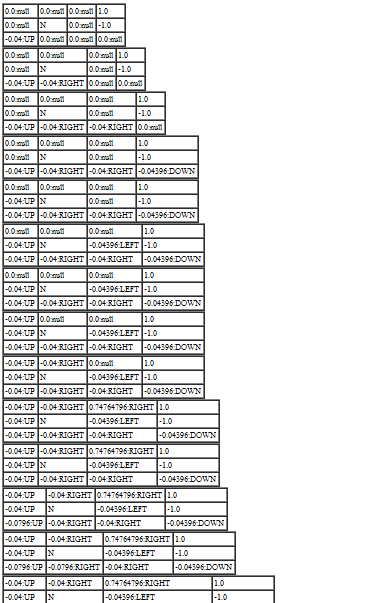
\includegraphics[width=0.90\textwidth]{Figures/Planning_Figure_2.png}
        \caption{Value Iteration Results}
        \label{fig:ValueIterationResults}
    \end{center}
\end{figure}

\begin{figure}[h!]
    \begin{center}
        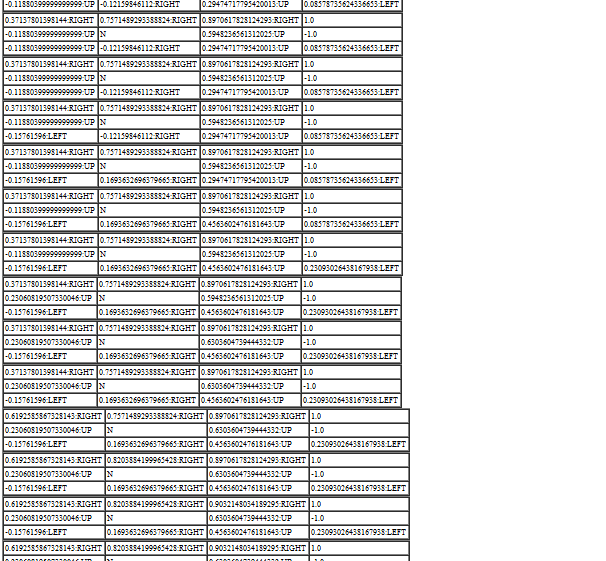
\includegraphics[width=0.95\textwidth]{Figures/Planning_Figure_3.png}
        \caption{Value Iteration Results}
        \label{fig:ValueIterationResults2}
    \end{center}
\end{figure}
\FloatBarrier
When the program reaches the maximum allowed error value it terminates. This
does not mean that the policy changes; policy will stabilize after a few
iterations based on the discount values we set, but the values in the value
iteration function will continuously change until it reaches the maximum allowed
error. We call this the epsilon factor. If we set the maximum allowed error
value to be large, then value iteration may terminate early.

We can see that in Figures~\ref{fig:ValueIterationResults} and
\ref{fig:ValueIterationResults2}, the values change continuously,
correspondingly action also
changes in accordance to the reward metrics. Since we do not start with the
initial set of policies, the value function will iteratively generate different
action sets that constitute the policy. After a few runs, the action set will
stabilize and we might call it a policy. It is important to let the
algorithm continue to run despite the stabilized policy. The algorithm may 
be stuck at a local minimum and may need some time
to get out of it.  Therefore, it is very important to carefully select the
discount factor.

From Figure~\ref{fig:ValueIterationResults2} we can see that the action set has
stabilized, and we
have a policy to reach the goal state. In reference to our problem statement if
an agent reaches a goal state, i.e. a simulated node/user who has an
artificially high trust values surrounded by nodes with very low trust value,
then there is an attack possibility and the decision is made not to transfer the
documents.

\subsubsection{Policy Iteration}
The policy iteration works similar to value iteration but the difference
mainly being that in policy iteration we start the algorithm with some random
policy (set of actions) and then use backward induction to improve the
policy. In the case of the
policy iteration the initial policy is assumed and the policy is constantly
evaluated and updated when the values are updated. As before, the values are the 
trust values of each node.  Equation \ref{eq:infinite_horizon2} is used in value 
iteration or infinite horizon.

\begin{equation} 
    \label{eq:infinite_horizon2}
    V_\pi(s) = T(s) + \beta \sum_{S'} M(s,\pi(s),s') \cdot V_\pi(s')
\end{equation}
The different parameters used in the above equation are the same as the ones in
the value iteration, the difference being that $\pi(s)$ represents a policy. The brief
description of the algorithm is as follows:
\begin{enumerate}
    \item Choose a random policy $\pi$
    \item Loop: 
        \begin{enumerate}
            \item Evaluate $V_\pi$ 
            \item For each $s$ in $S$, set improved policy
            \item Replace $\pi$ with $\pi^\prime$ 
        \end{enumerate}
        \item Until no improving action possible at any state
\end{enumerate}

The policy improvement is made using Equation~\ref{eq:policy_improvement}

\begin{equation} 
    \label{eq:policy_improvement}
    \pi'(s) = \operatorname*{argmax}_a \sum_{S'} T(s,a,s') \cdot V_\pi(s')
\end{equation}


\begin{figure}[h!]
    \begin{center}
        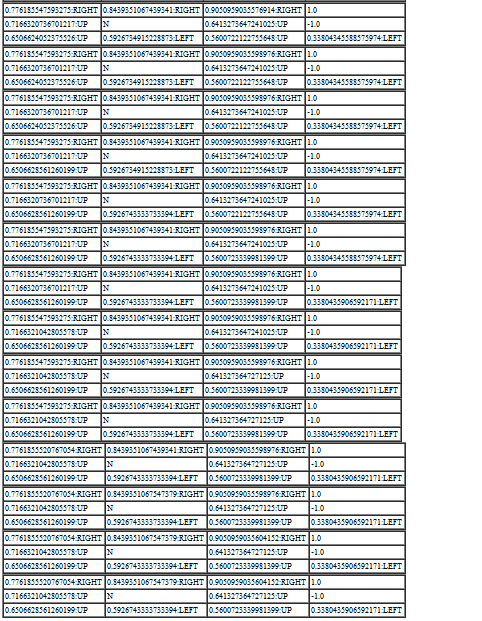
\includegraphics[width=0.95\textwidth]{Figures/Planning_Figure_4.png}
        \caption{Policy Iteration Results}
        \label{fig:PolicyIterationResults}
    \end{center}
\end{figure}

In Figure~\ref{fig:PolicyIterationResults} we can see the several runs of the policy iteration
algorithms. Here we start with the random policy and use the equations to update
the reward metrics of the every state and there updating the policy if any
better policy is found than one we started with or one that we have. We can see
the action sets stabilize at the end and hence arriving upon a policy that will
help us make the correct decision.

\FloatBarrier

\subsection{Running Time}

\begin{enumerate}
    \item From Figure Figures~\ref{fig:ValueIterationResults} we can see that the Value Iteration takes
more resources and running time compared to others. This is because of the fact
that there is no policy in the beginning. So the value iteration frames policies
as it proceeds. And of course the running time of the value iterations largely
depend on the maximum error value that we set.
    \item The policy iteration takes much less running time when we compare it to the
value iteration in this case. This is due to the fact that we start with an
arbitrary random policy. This will be a huge improvement because its like giving
a model to the function even though it may be wrong. The value will be computed
according to the initial policy setting. If it is correct it is unchanged, if
not then we change the policy and re-compute the value again.
\end{enumerate}
By running both policy iteration and value iteration within CloudAssure, we can conclude the following:
\begin{enumerate}
    \item CloudAssure is able to make informed decisions on data transfer decisions by
using good heuristics, which are simulated values for the data
classification and the trust values for the nodes/users
    \item The running time for
the algorithms is reasonable, we achieved convergence for a 12 state problem in
about a reasonable amount of time. Modification could be done if to scale the system.
\end{enumerate}
